\documentclass{article}
\usepackage{graphicx}
\usepackage{geometry}
\geometry{margin=1.5in}
\usepackage{hyperref}
\hypersetup{
    colorlinks=true,
    linkcolor=blue,
    filecolor=magenta,      
    urlcolor=cyan,
}


\begin{document}

\title{Realm.One}
\author{The Specification Document}

\maketitle
\begin{center}
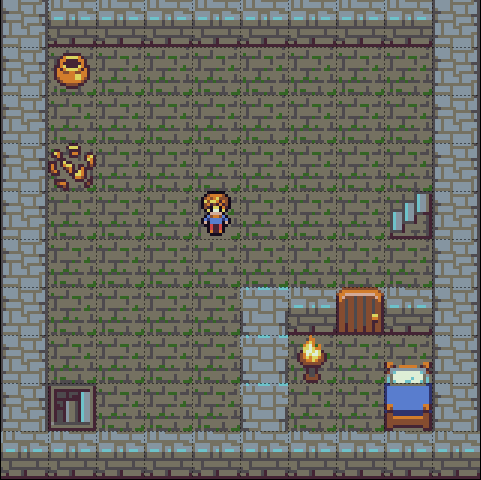
\includegraphics[scale=0.3]{ss.png}
\end{center}
\newpage

\section{Overview}
Realm one is an MMO that will serve to be the boiler plate for Worlds, which is a distributed MMO. If you don't know what that means, please check the code repository for Worlds \href{worldsmmo.com}{here}. The purpose of realm.one is to build a badass game that can demonstrate the power of distributed gaming on the Worlds platform, the vision is: anyone should be able to fork the realm.one repository and build their own game which can be integrated into a massive universe.

\section{Gameplay}
Realm.one will start off as a very simple game, I will outline an MVG (minimum viable game). Players should connect using the same rsa keys they use to validate their transactions on a blockchain, no passwords required. The MVG is:

\begin{itemize}
\item Player can walk around, throughout the map
\item Players can gain experience from killing monsters and doing quests
\item Players can obtain items
\item Players can see an interact with other players
\end{itemize}

\subsection{Storyline}
Maybe?

\section{Map}
The game map is built from tiles, each tile has a ``GID" and layer, a room is a ``.tmx" file, which contains all the tile placements and tile properties.  

\subsection{Static Tiles - L1/L2}
Static tiles are tiles which do not move or animate. There are situated on layers one 
and two of the ``.tmx" file. These are typically ``set and forget" they may have various parameters such as ``collision" which prevents monsters and players from walking over them.

\subsection{Movement Tiles - L3}
Movement tiles are tiles that indicate a change of map, such as stairs or hole. They contain a parameter that links to the next ``.tmx" map to move into.

\subsection{Object Tiles - L4}
Object tiles are tiles that may change but not move, such as a door (which can open or close). They contain various parameters that may indicate their status.

\subsection{Item Tiles - L5}
These are items that a player may pick up or move around.

\subsection{Monsters - L6}
Monsters move around and have various properties associate with them, hp etc...

\subsection{Players}
Player are special tiles that don't live on the tmx file.

\end{document}
